\renewcommand{\arraystretch}{1.5}
\section{Funkcje trygonometryczne}
    \begin{table}[htbp!]
        \footnotesize
        \centering
        \caption{Własności funkcji trygonometrycznych ($k \in \mathds{Z}$)}
        \label{tab:wlasnosci_funkcji_tryg}
        \vspace{3mm}
        \begin{tabular}{lcccc}
            Funckja & $sin\varphi$ & $cos\varphi$ & $tg\varphi$ & $ctg\varphi$\\
            \midrule
            Dziedzina & $\mathds{R}$ & $\mathds{R}$ & $\mathds{R}\setminus\{\frac{\pi}{2}+k\pi\}$ & $\mathds{R}\setminus\{k\pi\}$\\
            Przeciwdziedzina & $[-1;\,1]$ & $[-1;\,1]$ & $\mathds{R}$ & $\mathds{R}$\\
            \multirow{2}{*}{Ekstrema} & 1: $\{\frac{\pi}{2}+2k\pi\}$ & 1: $\{2k\pi\}$ & \multirow{2}{*}{-} & \multirow{2}{*}{-}\\
            & -1: $\{-\frac{\pi}{2}+2k\pi\}$ & -1: $\{\pi + 2k\pi\}$ & & \\
            Miejsca zerowe & $\{k\pi\}$ & $\{\frac{\pi}{2}+2k\pi\}$ & $\{k\pi\}$ & $\{\frac{\pi}{2}+2k\pi\}$\\
            Parzystość & nieparzysta & parzysta & nieparzysta & nieparzysta\\
            Ciągłość & $\mathds{R}$ & $\mathds{R}$ & $\mathds{R}\setminus\{\frac{\pi}{2}+k\pi\}$ & $\mathds{R}\setminus\{k\pi\}$\\
            \bottomrule
        \end{tabular}
    \end{table}
    
    \begin{figure}[p]
        \centering
        \caption{Wykres $sin\varphi$}
        \label{fig:wykres_sin}
        \vspace{3mm}
        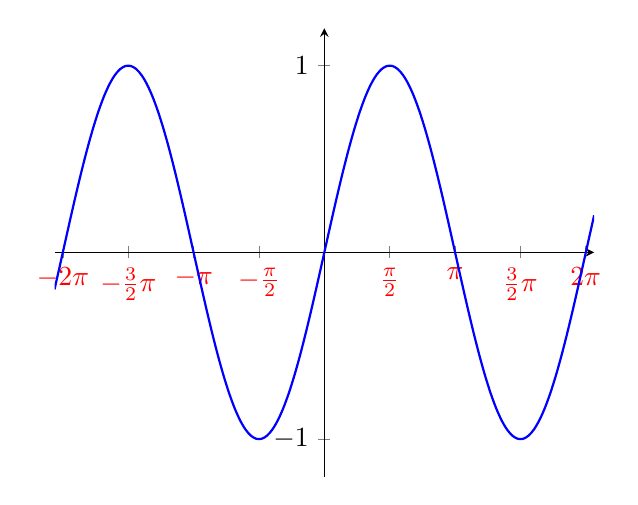
\begin{tikzpicture}
            \begin{axis}[
                    domain=-2*pi-0.2:2*pi+0.2,
                    axis lines=middle,
                    ymin=-1.2,
                    ymax=1.2,
                    ytick={-1,1},
                    xtick={-6.28, -4.71, -3.14,-1.57, 1.57, 3.14, 4.71, 6.28},
                    xticklabels={$-2\pi$, $-\frac{3}{2}\pi$, $-\pi$, $-\frac{\pi}{2}$, $\frac{\pi}{2}$, $\pi$, $\frac{3}{2}\pi$, $2\pi$},
                    xticklabel style={red}
                ]
                \addplot[blue,thick,solid,smooth,samples=100]{sin(deg(x))} 
                ;
            \end{axis}
        \end{tikzpicture}
    \end{figure}

    \begin{figure}[p]
        \centering
        \caption{Wykres $cos\varphi$}
        \label{fig:wykres_cos}
        \vspace{3mm}
        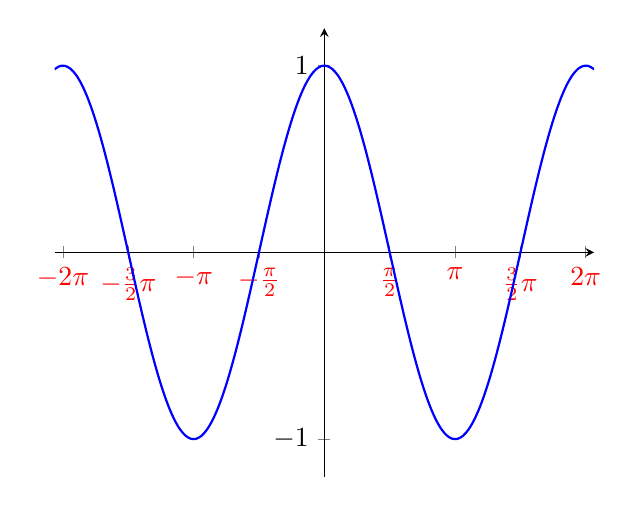
\begin{tikzpicture}
            \begin{axis}[
                    domain=-2*pi-0.2:2*pi+0.2,
                    axis lines=middle,
                    ymin=-1.2,
                    ymax=1.2,
                    ytick={-1,1},
                    xtick={-6.28, -4.71, -3.14,-1.57, 1.57, 3.14, 4.71, 6.28},
                    xticklabels={$-2\pi$, $-\frac{3}{2}\pi$, $-\pi$, $-\frac{\pi}{2}$, $\frac{\pi}{2}$, $\pi$, $\frac{3}{2}\pi$, $2\pi$},
                    xticklabel style={red}
                ]
                \addplot[blue,thick,solid,smooth,samples=100]{cos(deg(x))} 
                ;
            \end{axis}
        \end{tikzpicture}
    \end{figure}

    \begin{figure}[p]
        \centering
        \caption{Wykres $tg\varphi$}
        \label{fig:wykres_tg}
        \vspace{3mm}
        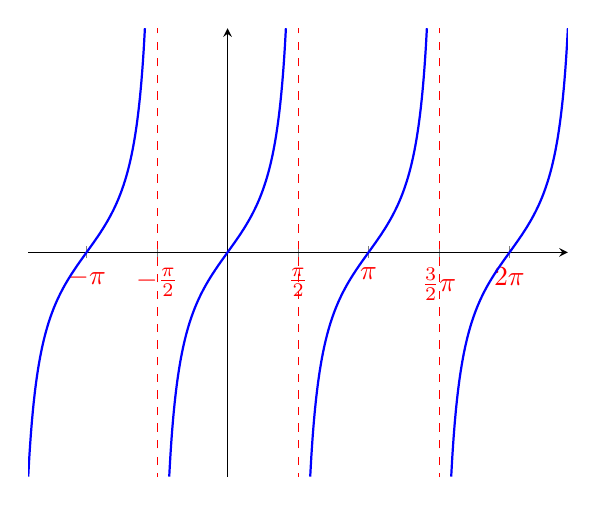
\begin{tikzpicture}
            \begin{axis}[
                    domain=-2*pi-0.2:2*pi+0.2,
                    axis lines=middle,
                    ytick={0},
                    xtick={-6.28, -4.71, -3.14,-1.57, 1.57, 3.14, 4.71, 6.28},
                    xticklabels={$-2\pi$, $-\frac{3}{2}\pi$, $-\pi$, $-\frac{\pi}{2}$, $\frac{\pi}{2}$, $\pi$, $\frac{3}{2}\pi$, $2\pi$},
                    xticklabel style={red}
                ]
                \draw[dashed,red] (-0.5*pi,-100) -- (-0.5*pi,100);
                \draw[dashed,red] (0.5*pi,-100) -- (0.5*pi,100);
                \draw[dashed,red] (1.5*pi,-100) -- (1.5*pi,100);
                \addplot[blue,thick,solid,smooth,samples=100,domain=-1*pi-1.3:-1*pi+1.3]{tan(deg(x))}; 
                \addplot[blue,thick,solid,smooth,samples=100,domain=1*pi-1.3:1*pi+1.3]{tan(deg(x))};
                \addplot[blue,thick,solid,smooth,samples=100,domain=-1.3:1.3]{tan(deg(x))}; 
                \addplot[blue,thick,solid,smooth,samples=100,domain=2*pi-1.3:2*pi+1.3]{tan(deg(x))};
                ;
            \end{axis}
        \end{tikzpicture}
    \end{figure}

    \begin{figure}[p]
        \centering
        \caption{Wykres $ctg\varphi$}
        \label{fig:wykres_ctg}
        \vspace{3mm}
        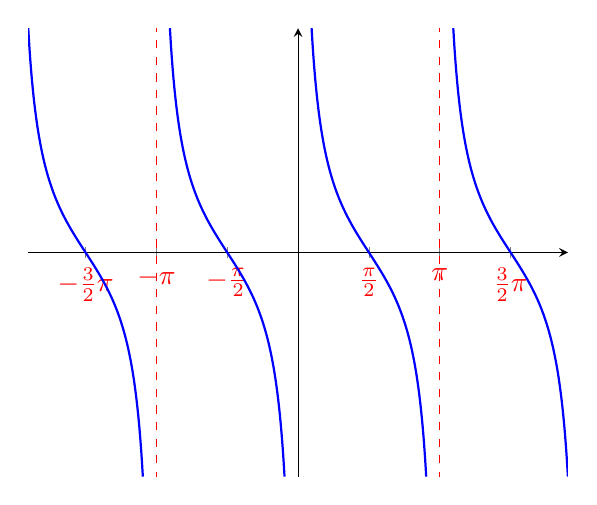
\begin{tikzpicture}
            \begin{axis}[
                    domain=-2*pi-0.2:2*pi+0.2,
                    axis lines=middle,
                    ytick={0},
                    xtick={-6.28, -4.71, -3.14,-1.57, 1.57, 3.14, 4.71, 6.28},
                    xticklabels={$-2\pi$, $-\frac{3}{2}\pi$, $-\pi$, $-\frac{\pi}{2}$, $\frac{\pi}{2}$, $\pi$, $\frac{3}{2}\pi$, $2\pi$},
                    xticklabel style={red}
                ]
                \draw[dashed,red] (-1*pi,-100) -- (-1*pi,100);
                \draw[dashed,red] (pi,-100) -- (pi,100);
                \draw[dashed,red] (2*pi,-100) -- (2*pi,100);
                \addplot[blue,thick,solid,smooth,samples=100,domain=-2*pi+0.3:-1*pi-0.3]{cot(deg(x))};
                \addplot[blue,thick,solid,smooth,samples=100,domain=-1*pi+0.3:-0.3]{cot(deg(x))}; 
                \addplot[blue,thick,solid,smooth,samples=100,domain=0.3:1*pi-0.3]{cot(deg(x))};
                \addplot[blue,thick,solid,smooth,samples=100,domain=pi+0.3:2*pi-0.3]{cot(deg(x))}; 
                ;
            \end{axis}
        \end{tikzpicture}
    \end{figure}

    \begin{table}[htbp]
        \footnotesize
        \centering
        \caption{Wzory redukcyjne funkcji trygonometrycznych}
        \label{tab:wzory_redukcyjne_tryg}
        \vspace{3mm}
        \begin{tabular}{c|c|cc|cc|cc|}
             & I ćwiartka & \multicolumn{2}{|c|}{II ćwiartka} & \multicolumn{2}{|c|}{III ćwiartka} & \multicolumn{2}{|c|}{III ćwiartka}\\
             \midrule
             \multirow{2}{*}{$\varphi$} & $90\degree - \alpha$ & $90\degree+\alpha$ & $180\degree - \alpha$ & $180\degree+\alpha$ & $270\degree - \alpha$ & $270\degree+\alpha$ & $360\degree-\alpha$ \\
             & $\frac{\pi}{2} - \alpha$ & $\frac{\pi}{2} + \alpha$ & $\pi - \alpha$ & $\pi + \alpha$ & $\frac{3}{2}\pi - \alpha$ & $\frac{3}{2}\pi + \alpha$ & $2\pi - \alpha$ \\ 
             \midrule
            $sin \varphi$ & $cos\alpha$ & $cos\alpha$ & $sin\alpha$ & $-sin\alpha$ & $-cos\alpha$ & $-cos\alpha$ & $-sin\alpha$ \\
            $cos \varphi$ & $sin\alpha$ & $-sin\alpha$ & $-cos\alpha$ & $-cos\alpha$ & $-sin\alpha$ & $cos\alpha$ & $sin\alpha$ \\
            $tg \varphi$ & $ctg\alpha$ & $-ctg\alpha$ & $-tg\alpha$ & $tg\alpha$ & $ctg\alpha$ & $-ctg\alpha$ & $-tg\alpha$ \\
            $ctg \varphi$ & $tg\alpha$ & $-tg\alpha$ & $-ctg\alpha$ & $ctg\alpha$ & $tg\alpha$ & $-tg\alpha$ & $-ctg\alpha$ \\
            \bottomrule
        \end{tabular}
    \end{table}

    \begin{table}[h!]
        \centering
        \caption{Wartości funkcji trygonometrycznych ważniejszych kątów}
        \label{tab:wartosci_tryg}
        \vspace{3mm}
        \begin{tabular}{cccccc}
            \multicolumn{2}{c}{$\varphi$} & \multirow{2}{*}{$sin\varphi$} & \multirow{2}{*}{$cos\varphi$} & \multirow{2}{*}{$tg\varphi$} & \multirow{2}{*}{$ctg\varphi$} \\
            deg & rad & & & &\\
            \midrule
            $0\degree$ & 0 & 0 & 1 & 0 & -\\
            $15\degree$ & $\frac{\pi}{12}$ & $\frac{\sqrt{6}-\sqrt{2}}{4}$ & $\frac{\sqrt{6}+\sqrt{2}}{4}$ & $2-\sqrt{3}$ & $2+\sqrt{3}$\\
            $30\degree$ & $\frac{\pi}{6}$ & $\frac{1}{2}$ & $\frac{\sqrt{3}}{2}$ & $\frac{\sqrt{3}}{3}$ & $\sqrt{3}$\\
            $45\degree$ & $\frac{\pi}{4}$ & $\frac{\sqrt{2}}{2}$ & $\frac{\sqrt{2}}{2}$ & $1$ & $1$\\
            $60\degree$ & $\frac{\pi}{3}$ & $\frac{\sqrt{3}}{2}$ & $\frac{1}{2}$ & $\sqrt{3}$ & $\frac{\sqrt{3}}{3}$\\
            $75\degree$ & $\frac{5\pi}{12}$ & $\frac{\sqrt{6}+\sqrt{2}}{4}$ & $\frac{\sqrt{6}-\sqrt{2}}{4}$ & $2+\sqrt{3}$ & $2-\sqrt{3}$\\
            $90\degree$ & $\frac{\pi}{2}$ & 1 & 0 & - & 0\\
            $180\degree$ & $\pi$ & 0 & -1 & 0 & -\\
            $270\degree$ & $\frac{3\pi}{2}$ & -1 & 0 & 1 & 0\\
            $360\degree$ & $2\pi$ & 0 & 1 & 0 & -\\
            \bottomrule
        \end{tabular}
    \end{table}

\renewcommand{\arraystretch}{1}
